% Options for packages loaded elsewhere
% Options for packages loaded elsewhere
\PassOptionsToPackage{unicode}{hyperref}
\PassOptionsToPackage{hyphens}{url}
\PassOptionsToPackage{dvipsnames,svgnames,x11names}{xcolor}
%
\documentclass[
  letterpaper,
  DIV=11,
  numbers=noendperiod]{scrartcl}
\usepackage{xcolor}
\usepackage[landscape, margin=0.5in, includehead, includefoot,
footskip=60pt, headsep=4pt]{geometry}
\usepackage{amsmath,amssymb}
\setcounter{secnumdepth}{-\maxdimen} % remove section numbering
\usepackage{iftex}
\ifPDFTeX
  \usepackage[T1]{fontenc}
  \usepackage[utf8]{inputenc}
  \usepackage{textcomp} % provide euro and other symbols
\else % if luatex or xetex
  \usepackage{unicode-math} % this also loads fontspec
  \defaultfontfeatures{Scale=MatchLowercase}
  \defaultfontfeatures[\rmfamily]{Ligatures=TeX,Scale=1}
\fi
\usepackage{lmodern}
\ifPDFTeX\else
  % xetex/luatex font selection
\fi
% Use upquote if available, for straight quotes in verbatim environments
\IfFileExists{upquote.sty}{\usepackage{upquote}}{}
\IfFileExists{microtype.sty}{% use microtype if available
  \usepackage[]{microtype}
  \UseMicrotypeSet[protrusion]{basicmath} % disable protrusion for tt fonts
}{}
\makeatletter
\@ifundefined{KOMAClassName}{% if non-KOMA class
  \IfFileExists{parskip.sty}{%
    \usepackage{parskip}
  }{% else
    \setlength{\parindent}{0pt}
    \setlength{\parskip}{6pt plus 2pt minus 1pt}}
}{% if KOMA class
  \KOMAoptions{parskip=half}}
\makeatother
% Make \paragraph and \subparagraph free-standing
\makeatletter
\ifx\paragraph\undefined\else
  \let\oldparagraph\paragraph
  \renewcommand{\paragraph}{
    \@ifstar
      \xxxParagraphStar
      \xxxParagraphNoStar
  }
  \newcommand{\xxxParagraphStar}[1]{\oldparagraph*{#1}\mbox{}}
  \newcommand{\xxxParagraphNoStar}[1]{\oldparagraph{#1}\mbox{}}
\fi
\ifx\subparagraph\undefined\else
  \let\oldsubparagraph\subparagraph
  \renewcommand{\subparagraph}{
    \@ifstar
      \xxxSubParagraphStar
      \xxxSubParagraphNoStar
  }
  \newcommand{\xxxSubParagraphStar}[1]{\oldsubparagraph*{#1}\mbox{}}
  \newcommand{\xxxSubParagraphNoStar}[1]{\oldsubparagraph{#1}\mbox{}}
\fi
\makeatother


\usepackage{longtable,booktabs,array}
\usepackage{calc} % for calculating minipage widths
% Correct order of tables after \paragraph or \subparagraph
\usepackage{etoolbox}
\makeatletter
\patchcmd\longtable{\par}{\if@noskipsec\mbox{}\fi\par}{}{}
\makeatother
% Allow footnotes in longtable head/foot
\IfFileExists{footnotehyper.sty}{\usepackage{footnotehyper}}{\usepackage{footnote}}
\makesavenoteenv{longtable}
\usepackage{graphicx}
\makeatletter
\newsavebox\pandoc@box
\newcommand*\pandocbounded[1]{% scales image to fit in text height/width
  \sbox\pandoc@box{#1}%
  \Gscale@div\@tempa{\textheight}{\dimexpr\ht\pandoc@box+\dp\pandoc@box\relax}%
  \Gscale@div\@tempb{\linewidth}{\wd\pandoc@box}%
  \ifdim\@tempb\p@<\@tempa\p@\let\@tempa\@tempb\fi% select the smaller of both
  \ifdim\@tempa\p@<\p@\scalebox{\@tempa}{\usebox\pandoc@box}%
  \else\usebox{\pandoc@box}%
  \fi%
}
% Set default figure placement to htbp
\def\fps@figure{htbp}
\makeatother





\setlength{\emergencystretch}{3em} % prevent overfull lines

\providecommand{\tightlist}{%
  \setlength{\itemsep}{0pt}\setlength{\parskip}{0pt}}



 


\KOMAoption{captions}{tableheading}
\pagestyle{fancy}
\fancyhf{}
\fancyhead[C]{
\raisebox{-15pt}[0pt][0pt]{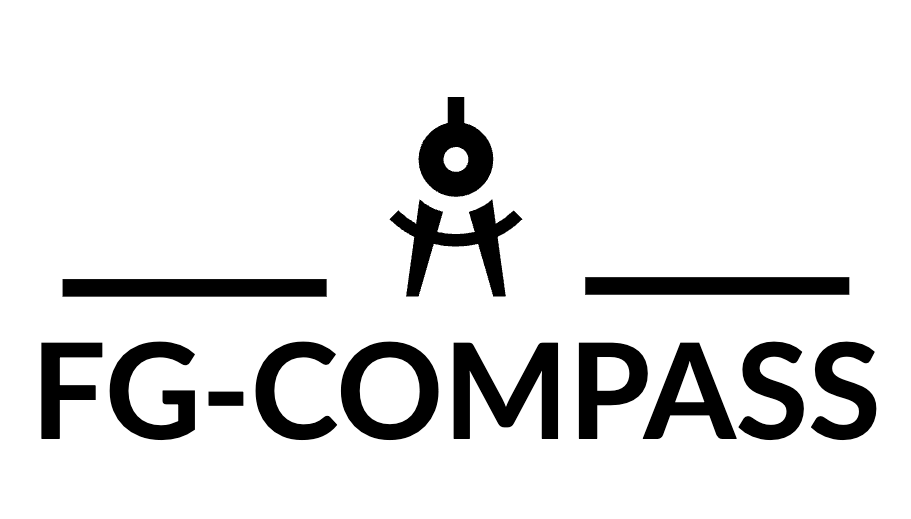
\includegraphics[height=40pt]{logo.png}}
}
\fancyfoot[C]{Furtado Jr, O., \& Gallagher, J. | FG-COMPASS - 2025 © All rights reserved | https://fgcompass.com | Page \thepage}
\renewcommand{\headrulewidth}{0pt}
\renewcommand{\footrulewidth}{0.4pt}
\addtolength{\textheight}{20pt}
\setlist[itemize]{topsep=0pt, partopsep=0pt, itemsep=0pt, parsep=0pt}
\makeatletter
\@ifpackageloaded{caption}{}{\usepackage{caption}}
\AtBeginDocument{%
\ifdefined\contentsname
  \renewcommand*\contentsname{Table of contents}
\else
  \newcommand\contentsname{Table of contents}
\fi
\ifdefined\listfigurename
  \renewcommand*\listfigurename{List of Figures}
\else
  \newcommand\listfigurename{List of Figures}
\fi
\ifdefined\listtablename
  \renewcommand*\listtablename{List of Tables}
\else
  \newcommand\listtablename{List of Tables}
\fi
\ifdefined\figurename
  \renewcommand*\figurename{Figure}
\else
  \newcommand\figurename{Figure}
\fi
\ifdefined\tablename
  \renewcommand*\tablename{Table}
\else
  \newcommand\tablename{Table}
\fi
}
\@ifpackageloaded{float}{}{\usepackage{float}}
\floatstyle{ruled}
\@ifundefined{c@chapter}{\newfloat{codelisting}{h}{lop}}{\newfloat{codelisting}{h}{lop}[chapter]}
\floatname{codelisting}{Listing}
\newcommand*\listoflistings{\listof{codelisting}{List of Listings}}
\makeatother
\makeatletter
\makeatother
\makeatletter
\@ifpackageloaded{caption}{}{\usepackage{caption}}
\@ifpackageloaded{subcaption}{}{\usepackage{subcaption}}
\makeatother
\usepackage{bookmark}
\IfFileExists{xurl.sty}{\usepackage{xurl}}{} % add URL line breaks if available
\urlstyle{same}
\hypersetup{
  colorlinks=true,
  linkcolor={blue},
  filecolor={Maroon},
  citecolor={Blue},
  urlcolor={Blue},
  pdfcreator={LaTeX via pandoc}}


\author{}
\date{}
\begin{document}


\setlength{\tabcolsep}{3pt}
\renewcommand{\arraystretch}{1.6}
\small
\vspace*{.5em} % Add vertical space after the header before the first table

% ---------------- Table 1 ----------------
\begin{tabular}{|p{5.5cm}|c|p{5.5cm}|c|c|*{9}{p{1.07cm}|}}
\hline
\multicolumn{5}{|c|}{\multirow{2}{*}{\centering \textbf{Locomotor-Hop}}} & \multicolumn{9}{c|}{\textbf{Student ID}} \\ 
\cline{6-14}
\multicolumn{5}{|c|}{} & & & & & & & & & \\
\hline
\multirow{4}{5.5cm}{\raggedright {\footnotesize Was the hanging leg's knee bent 90 degrees or less, with a vertical thigh?}} 
& \multirow{2}{*}{\footnotesize Y} 
& \multirow{2}{5cm}{\raggedright {\footnotesize Did the hanging leg's foot swing across the support leg's line like a pendulum?}} & {\footnotesize Y} & {\footnotesize Level 4} & & & & & & & & & \\
\cline{4-14}
& & & {\footnotesize N} & {\footnotesize Level 3} & & & & & & & & & \\
\cline{2-14}
& \multirow{2}{*}{\footnotesize N} & \multirow{2}{5cm}{\raggedright {\footnotesize Was the hanging leg held in front of the body?}} & {\footnotesize N} & {\footnotesize Level 2} & & & & & & & & & \\
\cline{4-14}
& & & {\footnotesize Y} & {\footnotesize Level 1} & & & & & & & & & \\
\hline
\end{tabular}

\vspace{.5em}

% ---------------- Table 2 ----------------
\begin{tabular}{@{}l@{\hspace{1.5em}}l@{}}
% LEFT COLUMN: bullet lists with adjusted vertical placement
\small
\raisebox{0pt}[0pt][0pt]{%
\begin{tabular}[t]{@{}p{8.4cm}@{}}
\vspace*{1ex} % small vertical nudge
\textbf{Set up} \\[-1em]
\begin{itemize}
  \item Create a 15-long traveling lane using cones.
  \item Tape starting and ending lines on the floor.
  \item Stand perpendicular to the traveling lane to see the starting and ending points.
  \item Place two cones (each end) 1 foot before the starting and ending lines.
\end{itemize}

\vspace{0.4em}
\textbf{Directions for performers} \\[-1em]
\begin{itemize}
  \item I want to see you hopping on one leg.
  \item Choose your preferred leg to hop.
  \item Start from that starting line and do not stop until you pass the ending line; then come back using the same leg.
  \item This is not a race; show your best form.
  \item Watch as I demonstrate.
\end{itemize}

\vspace{0.4em}
\textbf{Notes for examiners} \\[-1em]
\begin{itemize}
  \item Give the performer 4 trials (1st trial is for practice only).
  \item A behavior is considered present (answering YES) if observed in at least two trials.
\end{itemize}
\end{tabular}
}
&
% RIGHT COLUMN: full boxed 2x2 layout
\begin{tabular}[t]{|p{7.9cm}|p{7.9cm}|}
\hline
\textbf{Level 1$\rightarrow$} The suspended leg is held in front of the body. & \textbf{Level 2$\rightarrow$} The knee is flexed with the foot of the hanging leg held near the buttocks. \\
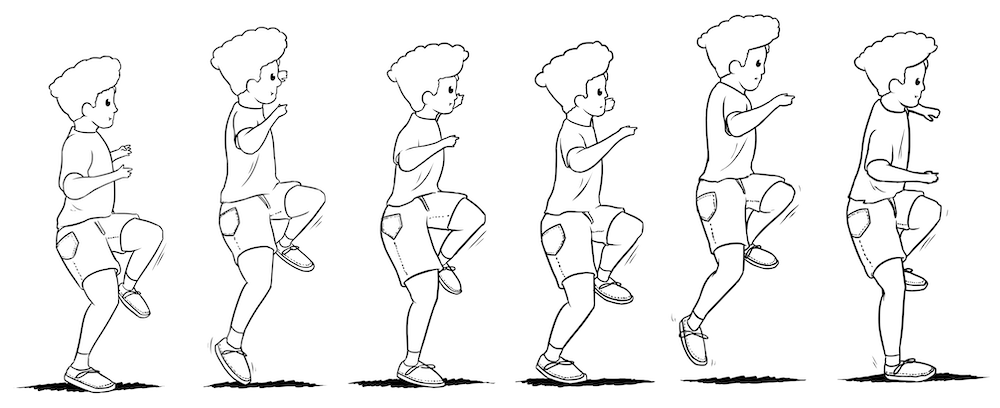
\includegraphics[width=0.9\linewidth]{static/images/loc-hop/ho1.png} & 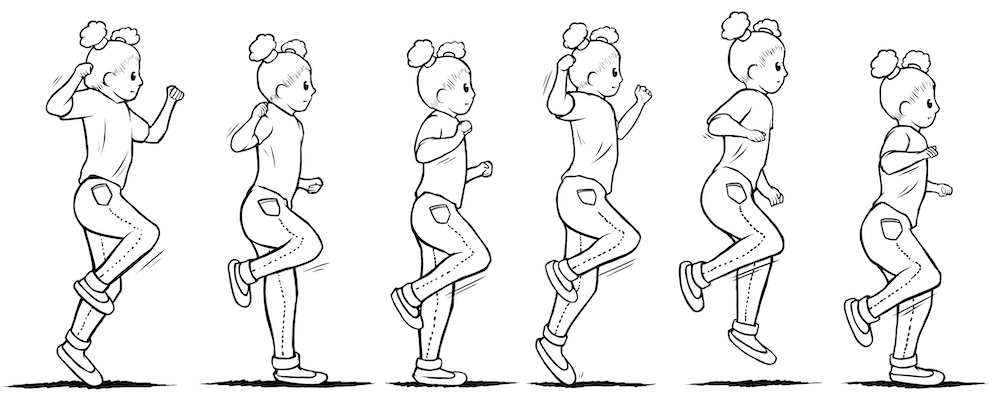
\includegraphics[width=0.9\linewidth]{static/images/loc-hop/ho2.png} \\
\hline
\textbf{Level 3$\rightarrow$} The hanging leg is held back with the thigh vertically. & \textbf{Level 4$\rightarrow$} Similar to Level 3, the foot of the hanging leg crosses the line of the support leg like a pendulum. \\
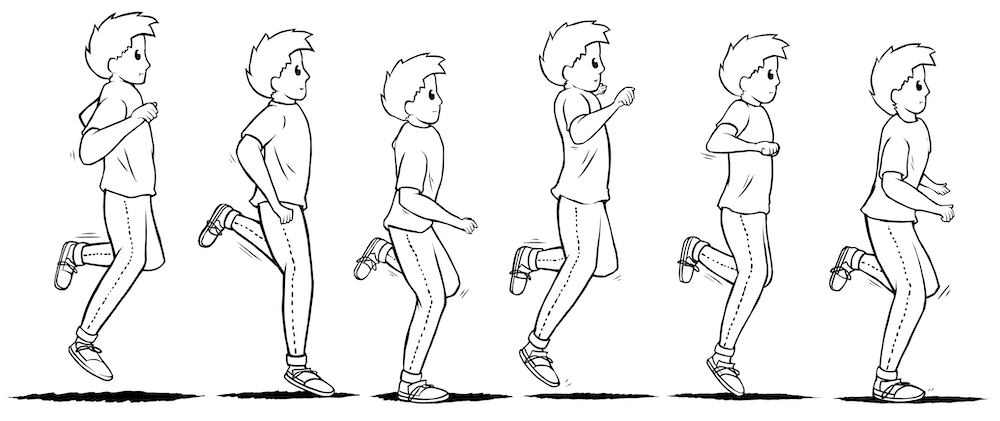
\includegraphics[width=0.9\linewidth]{static/images/loc-hop/ho3.png} & 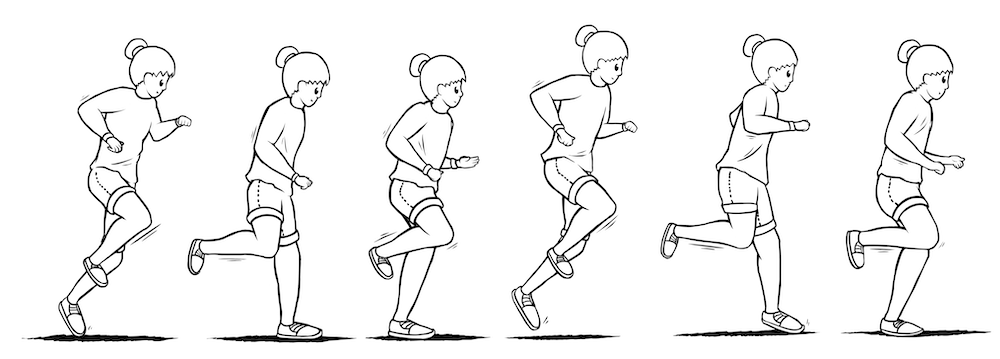
\includegraphics[width=0.9\linewidth]{static/images/loc-hop/ho4.png} \\
\hline
\end{tabular}
\end{tabular}

\newpage

\setlength{\tabcolsep}{3pt}
\renewcommand{\arraystretch}{1.6}
\small
\vspace*{.5em} % Add vertical space after the header before the first table

% ---------------- Table 1 ----------------
\begin{tabular}{|p{5.5cm}|c|p{5.5cm}|c|c|*{9}{p{1.07cm}|}}
\hline
\multicolumn{5}{|c|}{\multirow{2}{*}{\centering \textbf{Locomotor: Horizontal Jump}}} & \multicolumn{9}{c|}{\textbf{Student ID}} \\ 
\cline{6-14}
\multicolumn{5}{|c|}{} & & & & & & & & & \\
\hline
\multirow{4}{5.5cm}{\raggedright {\footnotesize Did the arms move forward \& upward upon takeoff and downward at landing?}} 
& \multirow{2}{*}{\footnotesize Y} 
& \multirow{2}{5cm}{\raggedright {\footnotesize Did the hands exceed the height of the head at liftoff?}} & {\footnotesize Y} & {\footnotesize Level 4} & & & & & & & & & \\
\cline{4-14}
& & & {\footnotesize N} & {\footnotesize Level 3} & & & & & & & & & \\
\cline{2-14}
& \multirow{2}{*}{\footnotesize N} & \multirow{2}{5cm}{\raggedright {\footnotesize Was the takeoff/landing executed on one foot?}} & {\footnotesize N} & {\footnotesize Level 2} & & & & & & & & & \\
\cline{4-14}
& & & {\footnotesize Y} & {\footnotesize Level 1} & & & & & & & & & \\
\hline
\end{tabular}

\vspace{.5em}

% ---------------- Table 2 ----------------
\begin{tabular}{@{}l@{\hspace{1.5em}}l@{}}
% LEFT COLUMN: bullet lists with adjusted vertical placement
\small
\raisebox{0pt}[0pt][0pt]{%
\begin{tabular}[t]{@{}p{8.4cm}@{}}
\vspace*{1ex} % small vertical nudge
\textbf{Set up} \\[-1em]
\begin{itemize}
    \item Tape two parallel lines on the floor two feet apart.
    \item Stand perpendicular to the jumping action facing the side of the child.
\end{itemize}

\vspace{0.4em}
\textbf{Directions for performers} \\[-1em]
\begin{itemize}
    \item I want to see you jumping forward over the second line and using both feet.
    \item Walk up to the first line and stop completely.
    \item Then, jump as far as you can over the second line.
    \item Use both feet when taking off and landing.
    \item Then, walk back to the starting point and do it again.
    \item There is no rush; show your best jump.
    \item Watch as I demonstrate.
\end{itemize}

\vspace{0.4em}
\textbf{Notes for examiners} \\[-1em]
\begin{itemize}
    \item Give the performer 4 trials (1st trial is for practice only).
    \item The child must stop completely behind the line before jumping.
\end{itemize}
\end{tabular}
}
&
% RIGHT COLUMN: full boxed 2x2 layout
\begin{tabular}[t]{|p{7.9cm}|p{7.9cm}|}
\hline
\textbf{Level 1$\rightarrow$} The arm action is inconsistent with no defined pattern, sometimes even motionless. The takeoff and/or landing is executed on one foot. & \textbf{Level 2$\rightarrow$} The arm action may still be inconsistent, but the takeoff/landing is executed on both feet. \\
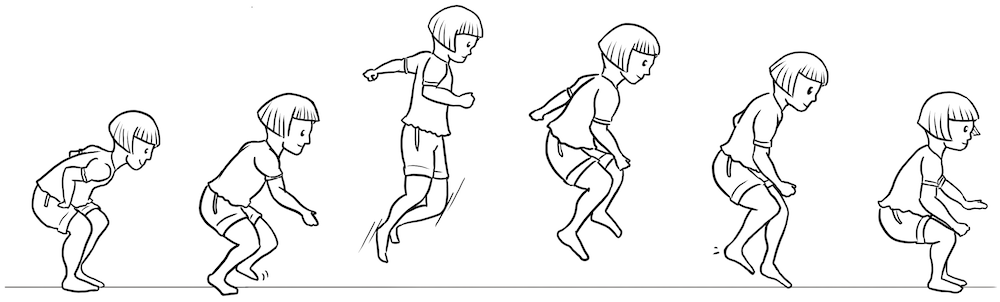
\includegraphics[width=0.9\linewidth]{static/images/loc-hj/hj1.png} & 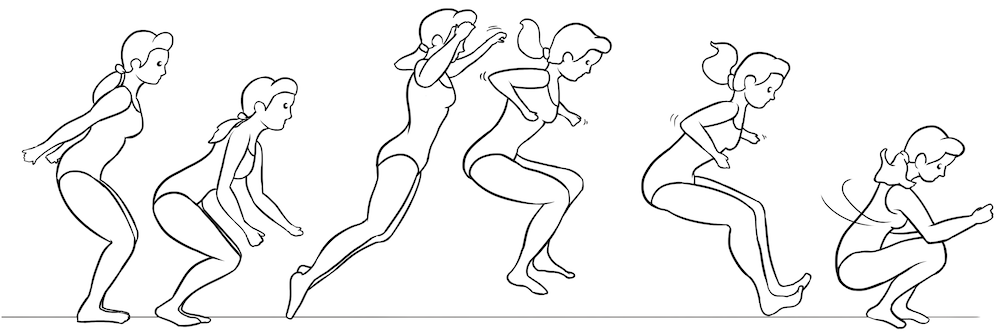
\includegraphics[width=0.9\linewidth]{static/images/loc-hj/hj2.png} \\
\hline
\textbf{Level 3$\rightarrow$} The arms move forward and upward during takeoff and then downward at landing. But the hands do not exceed the height of the head at liftoff. & \textbf{Level 4$\rightarrow$} A pattern similar to Level 3, but the hands are high above the head during the liftoff. \\
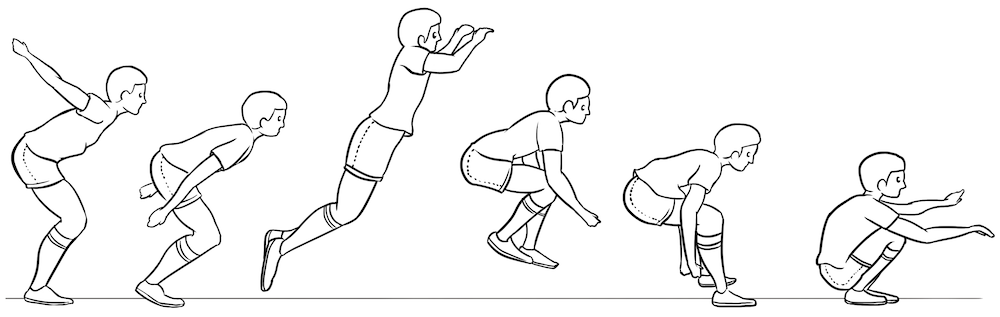
\includegraphics[width=0.9\linewidth]{static/images/loc-hj/hj3.png} & 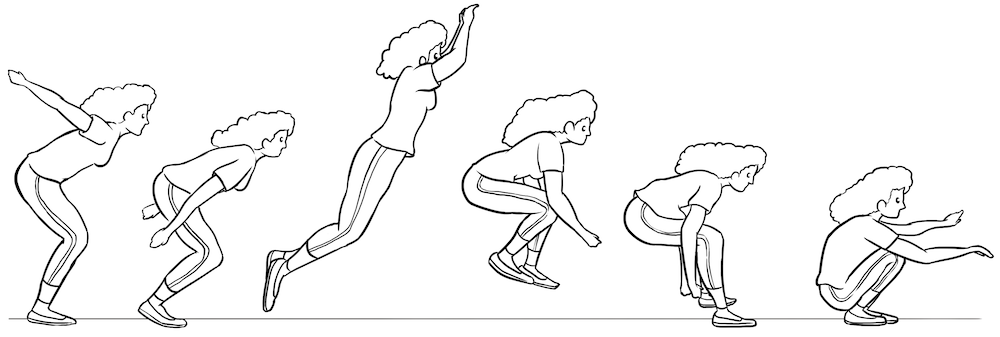
\includegraphics[width=0.9\linewidth]{static/images/loc-hj/hj4.png} \\
\hline
\end{tabular}
\end{tabular}

\newpage

\setlength{\tabcolsep}{3pt}
\renewcommand{\arraystretch}{1.6}
\small
\vspace*{.5em} % Add vertical space after the header before the first table

% ---------------- Table 1 ----------------
\begin{tabular}{|p{5.5cm}|c|p{5.5cm}|c|c|*{9}{p{1.07cm}|}}
\hline
\multicolumn{5}{|c|}{\multirow{2}{*}{\centering \textbf{Locomotor: Skip}}} & \multicolumn{9}{c|}{\textbf{Student ID}} \\ 
\cline{6-14}
\multicolumn{5}{|c|}{} & & & & & & & & & \\
\hline
\multirow{4}{5.5cm}{\raggedright {\footnotesize Did the arms move rhythmically in opposition to the legs?}} 
& \multirow{2}{*}{\footnotesize Y} 
& \multirow{2}{5cm}{\raggedright {\footnotesize Was there a low vertical lift on the hop?}} & {\footnotesize Y} & {\footnotesize Level 4} & & & & & & & & & \\
\cline{4-14}
& & & {\footnotesize N} & {\footnotesize Level 3} & & & & & & & & & \\
\cline{2-14}
& \multirow{2}{*}{\footnotesize N} & \multirow{2}{5cm}{\raggedright {\footnotesize Was there a break in the rhythm caused by a double hop or step?}} & {\footnotesize N} & {\footnotesize Level 2} & & & & & & & & & \\
\cline{4-14}
& & & {\footnotesize Y} & {\footnotesize Level 1} & & & & & & & & & \\
\hline
\end{tabular}

\vspace{.5em}

% ---------------- Table 2 ----------------
\begin{tabular}{@{}l@{\hspace{1.5em}}l@{}}
% LEFT COLUMN: bullet lists with adjusted vertical placement
\small
\raisebox{0pt}[0pt][0pt]{%
\begin{tabular}[t]{@{}p{8.4cm}@{}}
\vspace*{1ex} % small vertical nudge
\textbf{Set up} \\[-1em]
\begin{itemize}
    \item Create a 15-long traveling lane using cones.
    \item Tape starting and ending lines on the floor.
    \item Stand perpendicular to the traveling lane to see the starting and ending points.
    \item Place two cones (each end) 1 foot before the starting and ending lines.
\end{itemize}

\vspace{0.4em}
\textbf{Directions for performers} \\[-1em]
\begin{itemize}
    \item I want to see you skipping.
    \item Start from that starting line, and do not stop until you pass the ending line.
    \item This is not a race; show your best form.
    \item Watch as I demonstrate.
\end{itemize}

\vspace{0.4em}
\textbf{Notes for examiners} \\[-1em]
\begin{itemize}
    \item Give the performer 4 trials (1st trial is for practice only).
    \item A behavior is considered present (answering YES) if observed in at least two trials.
\end{itemize}
\end{tabular}
}
&
% RIGHT COLUMN: full boxed 2x2 layout
\begin{tabular}[t]{|p{7.9cm}|p{7.9cm}|}
\hline
\textbf{Level 1$\rightarrow$} The arm action is inconsistent, with no defined pattern. A double hop or step affects the rhythm. & \textbf{Level 2$\rightarrow$} The arm motion may improve but is still inconsistent and often motionless. The action of the feet is well coordinated and not affected by a double hop or step. \\
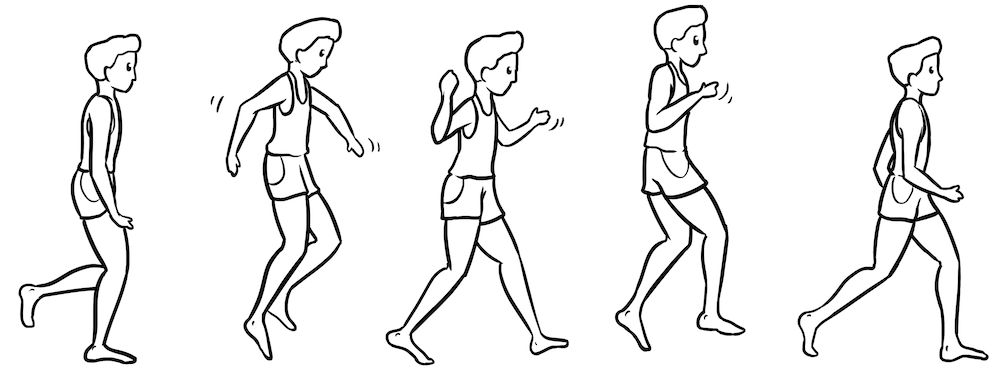
\includegraphics[width=0.9\linewidth]{static/images/loc-skip/sk1.png} & 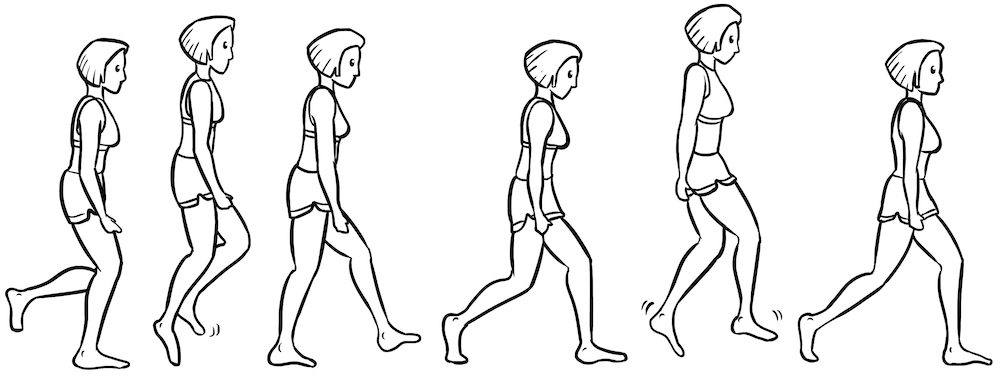
\includegraphics[width=0.9\linewidth]{static/images/loc-skip/sk2.png} \\
\hline
\textbf{Level 3$\rightarrow$} Arms move rhythmically in opposition to the legs, but the hop has an exaggerated vertical lift. & \textbf{Level 4$\rightarrow$} The arms move rhythmically in opposition to the legs, and the vertical lift on the hop is low. \\
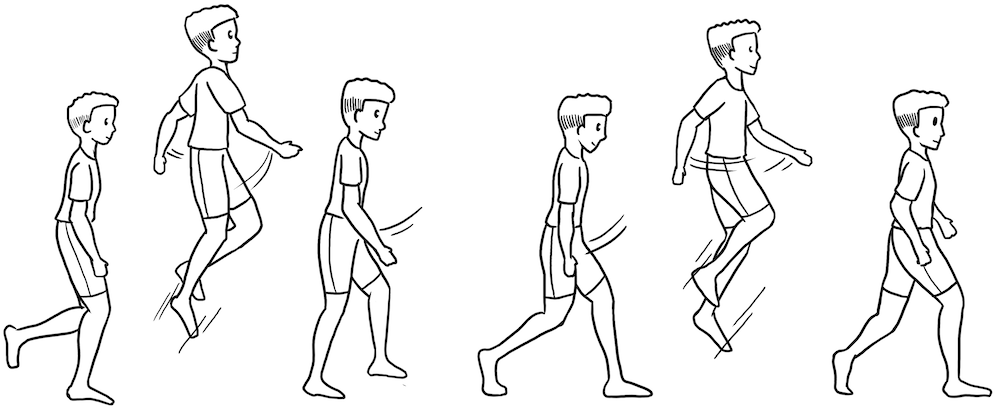
\includegraphics[width=0.9\linewidth]{static/images/loc-skip/sk3.png} & 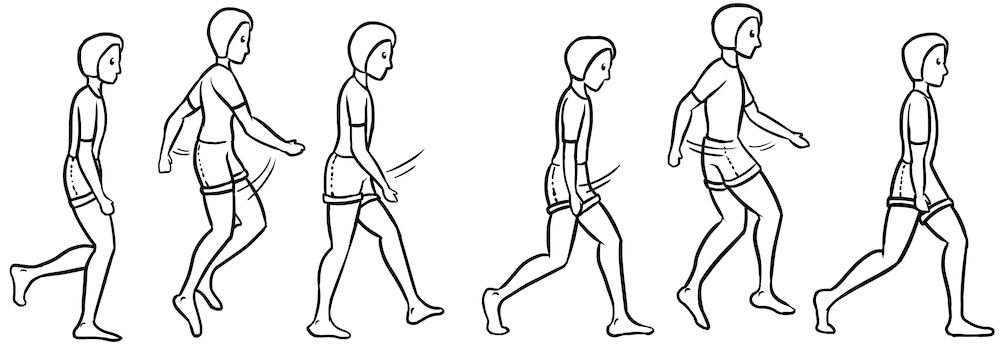
\includegraphics[width=0.9\linewidth]{static/images/loc-skip/sk4.png} \\
\hline
\end{tabular}
\end{tabular}

\newpage

\setlength{\tabcolsep}{3pt}
\renewcommand{\arraystretch}{1.6}
\small
\vspace*{.5em} % Add vertical space after the header before the first table

% ---------------- Table 1 ----------------
\begin{tabular}{|p{5.5cm}|c|p{5.5cm}|c|c|*{9}{p{1.07cm}|}}
\hline
\multicolumn{5}{|c|}{\multirow{2}{*}{\centering \textbf{Locomotor: Vertical Jump}}} & \multicolumn{9}{c|}{\textbf{Student ID}} \\ 
\cline{6-14}
\multicolumn{5}{|c|}{} & & & & & & & & & \\
\hline
\multirow{4}{5.5cm}{\raggedright {\footnotesize Did the arms move backward during preparation?}} 
& \multirow{2}{*}{\footnotesize Y} 
& \multirow{2}{5cm}{\raggedright {\footnotesize Did one arm reach upward at the flight’s peak while the other swung downward?}} & {\footnotesize Y} & {\footnotesize Level 4} & & & & & & & & & \\
\cline{4-14}
& & & {\footnotesize N} & {\footnotesize Level 3} & & & & & & & & & \\
\cline{2-14}
& \multirow{2}{*}{\footnotesize N} & \multirow{2}{5cm}{\raggedright {\footnotesize Was the takeoff/landing executed on one foot?}} & {\footnotesize N} & {\footnotesize Level 2} & & & & & & & & & \\
\cline{4-14}
& & & {\footnotesize Y} & {\footnotesize Level 1} & & & & & & & & & \\
\hline
\end{tabular}

\vspace{.5em}

% ---------------- Table 2 ----------------
\begin{tabular}{@{}l@{\hspace{1.5em}}l@{}}
% LEFT COLUMN: bullet lists with adjusted vertical placement
\small
\raisebox{0pt}[0pt][0pt]{%
\begin{tabular}[t]{@{}p{8.4cm}@{}}
\vspace*{1ex} % small vertical nudge
\textbf{Set up} \\[-1em]
\begin{itemize}
    \item Tape four parallel lines on the wall two feet apart.
    \item Stand perpendicular to the jumping action, facing the side of the performer.
    \item Ask the child to stand sideways with the dominant arm facing the wall.
\end{itemize}

\vspace{0.4em}
\textbf{Directions for performers} \\[-1em]
\begin{itemize}
    \item I want to see you jump high.
    \item Walk up to the wall and stand sideways.
    \item When I say so, jump up and touch the highest point on the wall using your dominant hand.
    \item Use both feet when taking off and landing.
    \item Then, get back to the starting position.
    \item There is no rush; show your best jump.
    \item Watch as I demonstrate.
\end{itemize}

\vspace{0.4em}
\textbf{Notes for examiners} \\[-1em]
\begin{itemize}
    \item Give the performer four trials (1st trial is for practice only).
    \item Ask the child to show the hand he/she writes with. That will help determine the dominant hand.
\end{itemize}
\end{tabular}
}
&
% RIGHT COLUMN: full boxed 2x2 layout
\begin{tabular}[t]{|p{7.9cm}|p{7.9cm}|}
\hline
\textbf{Level 1$\rightarrow$} The arms don't move to the rear before taking off; the child takes off and/or lands with one foot. & \textbf{Level 2$\rightarrow$} Arms don't move to the rear before takeoff; takeoff and landing occur with both feet. \\
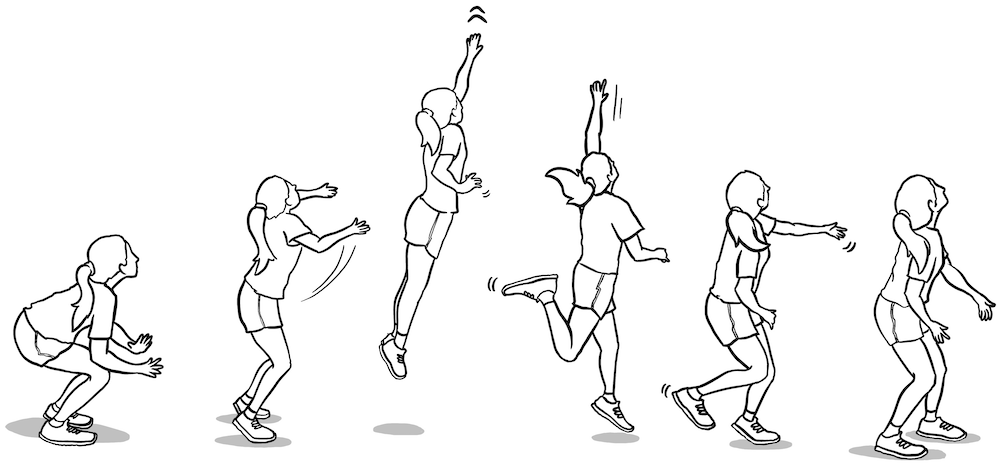
\includegraphics[width=0.9\linewidth]{static/images/loc-vj/vj1.png} & 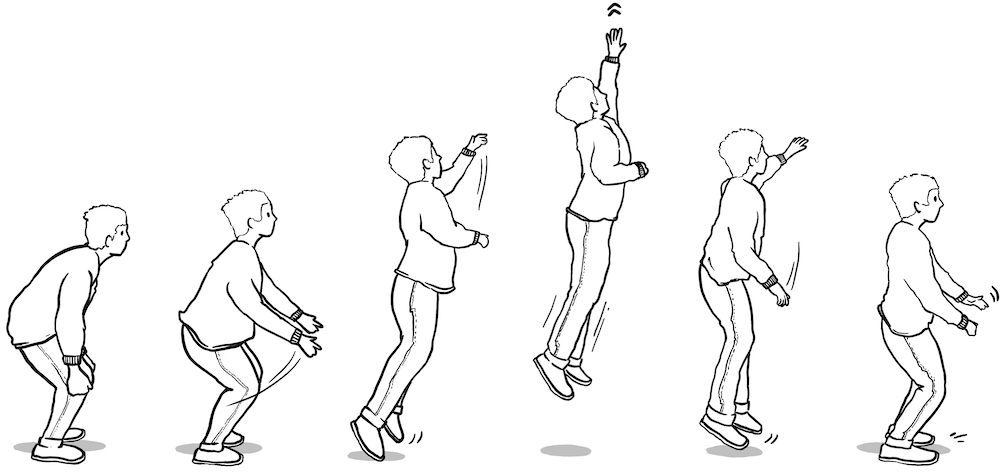
\includegraphics[width=0.9\linewidth]{static/images/loc-vj/vj2.png} \\
\hline
\textbf{Level 3$\rightarrow$} Arms move to the rear before taking off, but only the reaching arm reaches up. & \textbf{Level 4$\rightarrow$} Arms move to the rear before taking off; both arms reach up, with the non-reaching arm moving down at the peak of the flight. \\
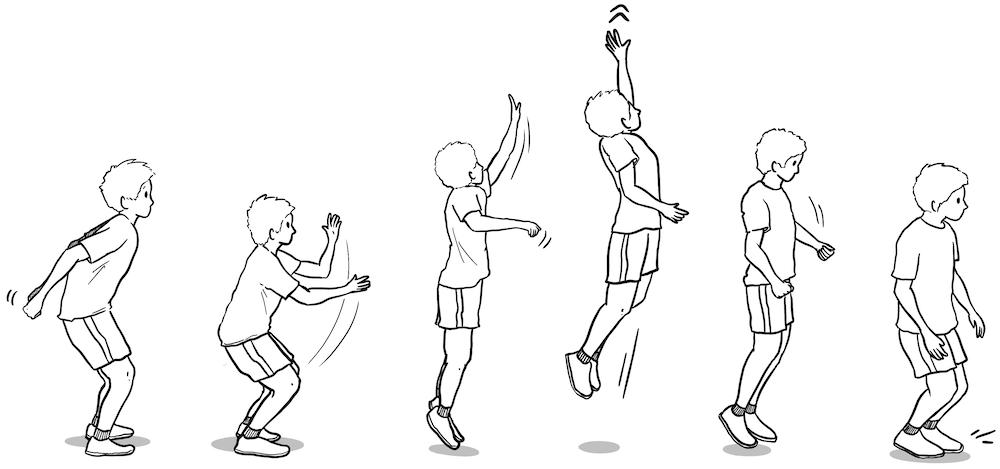
\includegraphics[width=0.9\linewidth]{static/images/loc-vj/vj3.png} & 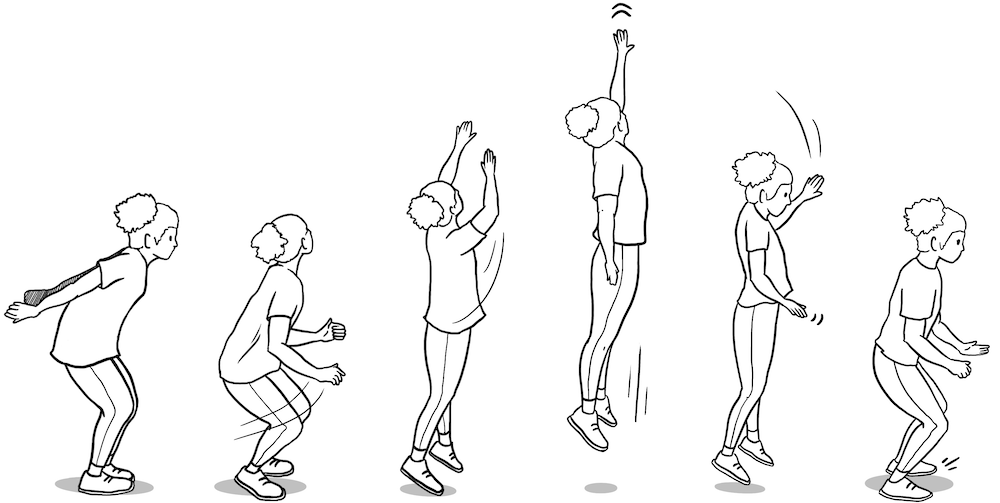
\includegraphics[width=0.9\linewidth]{static/images/loc-vj/vj4.png} \\
\hline
\end{tabular}
\end{tabular}

\newpage

\setlength{\tabcolsep}{3pt}
\renewcommand{\arraystretch}{1.6}
\small
\vspace*{.5em} % Add vertical space after the header before the first table

% ---------------- Table 1 ----------------
\begin{tabular}{|p{5.5cm}|c|p{5.5cm}|c|c|*{9}{p{1.07cm}|}}
\hline
\multicolumn{5}{|c|}{\multirow{2}{*}{\centering \textbf{Locomotor: Gallop}}} & \multicolumn{9}{c|}{\textbf{Student ID}} \\ 
\cline{6-14}
\multicolumn{5}{|c|}{} & & & & & & & & & \\
\hline
\multirow{4}{5.5cm}{\raggedright {\footnotesize Was the action smooth (not choppy) and performed at a moderate speed?}} 
& \multirow{2}{*}{\footnotesize Y} 
& \multirow{2}{5cm}{\raggedright {\footnotesize Did the arms move in unison, upward during takeoff and downward during landing?}} & {\footnotesize Y} & {\footnotesize Level 4} & & & & & & & & & \\
\cline{4-14}
& & & {\footnotesize N} & {\footnotesize Level 3} & & & & & & & & & \\
\cline{2-14}
& \multirow{2}{*}{\footnotesize N} & \multirow{2}{5cm}{\raggedright {\footnotesize Did the trailing foot land in front of the leading foot?}} & {\footnotesize N} & {\footnotesize Level 2} & & & & & & & & & \\
\cline{4-14}
& & & {\footnotesize Y} & {\footnotesize Level 1} & & & & & & & & & \\
\hline
\end{tabular}

\vspace{.5em}

% ---------------- Table 2 ----------------
\begin{tabular}{@{}l@{\hspace{1.5em}}l@{}}
% LEFT COLUMN: bullet lists with adjusted vertical placement
\small
\raisebox{0pt}[0pt][0pt]{%
\begin{tabular}[t]{@{}p{8.4cm}@{}}
\vspace*{1ex} % small vertical nudge
\textbf{Set up} \\[-1em]
\begin{itemize}
    \item Create a 15-long traveling lane using cones.
    \item Tape starting and ending lines on the floor.
    \item Stand perpendicular to the traveling lane to see the starting and ending points.
    \item Place two cones (each end) 1 foot before the starting and ending lines.
\end{itemize}

\vspace{0.4em}
\textbf{Directions for performers} \\[-1em]
\begin{itemize}
    \item I want to see you galloping.
    \item Start from the starting line and do not stop until you pass the ending line.
    \item This is not a race, show your best form.
    \item Watch as I demonstrate.
\end{itemize}

\vspace{0.4em}
\textbf{Notes for examiners} \\[-1em]
\begin{itemize}
    \item Give the performer four trials (1st trial is for practice only).
\end{itemize}
\end{tabular}
}
&
% RIGHT COLUMN: full boxed 2x2 layout
\begin{tabular}[t]{|p{7.9cm}|p{7.9cm}|}
\hline
\textbf{Level 1$\rightarrow$} The action is not smooth and seems choppy/stiff. It is often done at a fast tempo, and the trailing foot (the foot that follows) lands in front of the leading foot. & \textbf{Level 2$\rightarrow$} Still not a smooth action, but while the trailing foot may cross the leading foot during airborne action, it does not land in front of the leading foot. \\
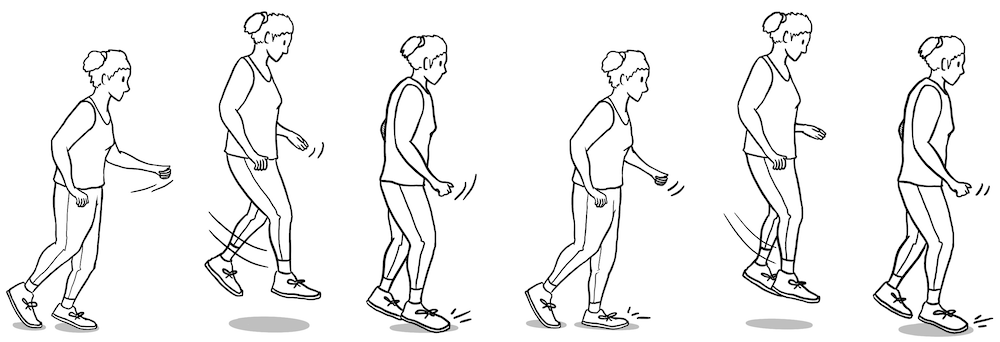
\includegraphics[width=0.9\linewidth]{static/images/loc-gallop/ga1.png} & 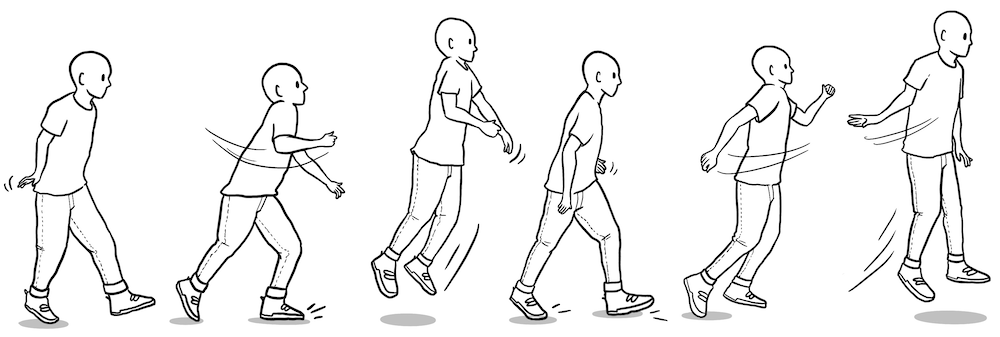
\includegraphics[width=0.9\linewidth]{static/images/loc-gallop/ga2.png} \\
\hline
\textbf{Level 3$\rightarrow$} The action is smooth, rhythmical, and done at a moderate tempo, but the arm action lacks a defined pattern. & \textbf{Level 4$\rightarrow$} The action is smooth, rhythmical, and done at a moderate speed; the arms (elbows) are lifted to waist Level at takeoff and moved down at landing. \\
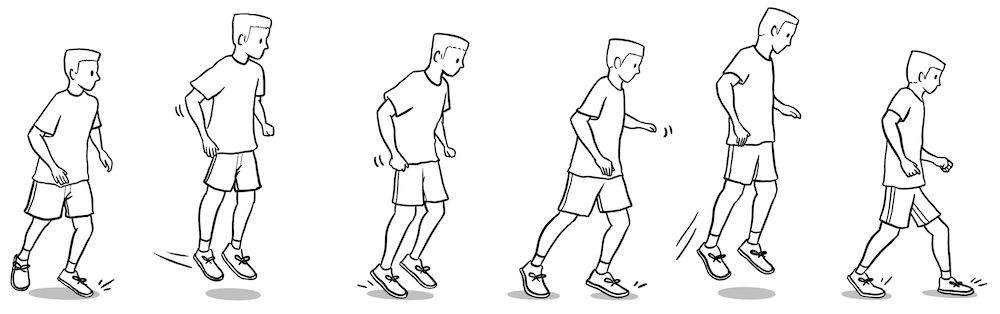
\includegraphics[width=0.9\linewidth]{static/images/loc-gallop/ga3.png} & 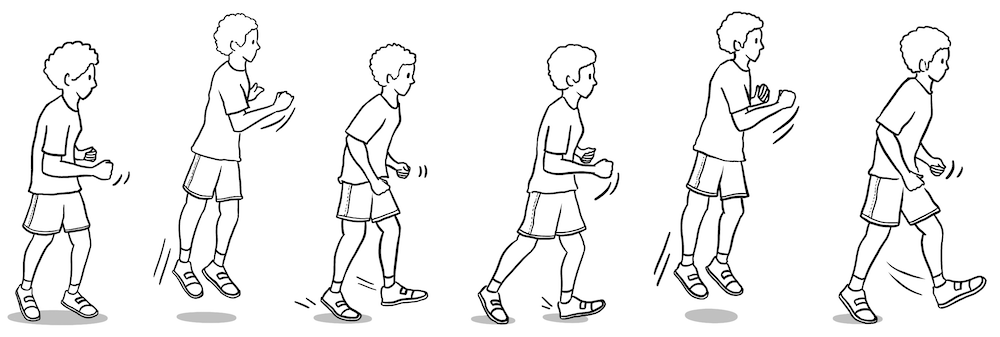
\includegraphics[width=0.9\linewidth]{static/images/loc-gallop/ga4.png} \\
\hline
\end{tabular}
\end{tabular}

\newpage

\setlength{\tabcolsep}{3pt}
\renewcommand{\arraystretch}{1.6}
\small
\vspace*{.5em} % Add vertical space after the header before the first table

% ---------------- Table 1 ----------------
\begin{tabular}{|p{5.5cm}|c|p{5.5cm}|c|c|*{9}{p{1.07cm}|}}
\hline
\multicolumn{5}{|c|}{\multirow{2}{*}{\centering \textbf{Manipulative: Overhand Throw}}} & \multicolumn{9}{c|}{\textbf{Student ID}} \\ 
\cline{6-14}
\multicolumn{5}{|c|}{} & & & & & & & & & \\
\hline
\multirow{4}{5.5cm}{\raggedright {\footnotesize Did the trunk rotate to the side of the throw during preparation?}} 
& \multirow{2}{*}{\footnotesize Y} 
& \multirow{2}{5.5cm}{\raggedright {\footnotesize Was there a long step opposite the throwing arm?}} & {\footnotesize Y} & {\footnotesize Level 4} & & & & & & & & & \\
\cline{4-14}
& & & {\footnotesize N} & {\footnotesize Level 3} & & & & & & & & & \\
\cline{2-14}
& \multirow{2}{*}{\footnotesize N} & \multirow{2}{6cm}{\raggedright {\footnotesize Did the child fail to step forward?}} & {\footnotesize N} & {\footnotesize Level 2} & & & & & & & & & \\
\cline{4-14}
& & & {\footnotesize Y} & {\footnotesize Level 1} & & & & & & & & & \\
\hline
\end{tabular}

\vspace{.5em}

% ---------------- Table 2 ----------------
\begin{tabular}{@{}l@{\hspace{1.5em}}l@{}}
% LEFT COLUMN: bullet lists with adjusted vertical placement
\small
\raisebox{0pt}[0pt][0pt]{%
\begin{tabular}[t]{@{}p{8.4cm}@{}}
\vspace*{1ex} % small vertical nudge
\textbf{Set up} \\[-1em]
\begin{itemize}
    \item Tape a line 20 feet from the wall on the floor.
    \item Stand about 10 feet from the examinee to get a side view of the action.
    \item Place a bucket containing several bean bags three feet ahead of the line.
\end{itemize}

\vspace{0.4em}
\textbf{Directions for performers} \\[-1em]
\begin{itemize}
    \item I want to see your throw.
    \item Walk up to the bucket, grab one beanbag, and throw it as hard as you can against the wall without stepping over the line.
    \item Then do it three more times.
    \item Watch as I demonstrate.
\end{itemize}

\vspace{0.4em}
\textbf{Notes for examiners} \\[-1em]
\begin{itemize}
    \item Give the performer four trials (the first trial is for practice only).
    \item Do not allow performers to step over the line.
\end{itemize}
\end{tabular}
}
&
% RIGHT COLUMN: full boxed 2x2 layout
\begin{tabular}[t]{|p{7.9cm}|p{7.9cm}|}
\hline
\textbf{Level 1$\rightarrow$} The trunk faces the target, and there is no step forward. Jumping up and down is not considered a step forward. & \textbf{Level 2$\rightarrow$} Minimal or no trunk rotation is observed during the preparatory phase. However, a forward step is taken, using either foot. \\
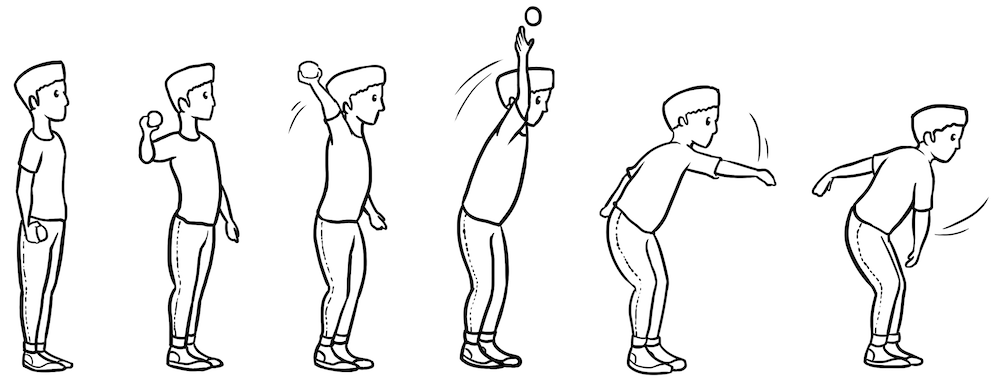
\includegraphics[width=0.9\linewidth]{static/images/man-ot/ot1.png} & 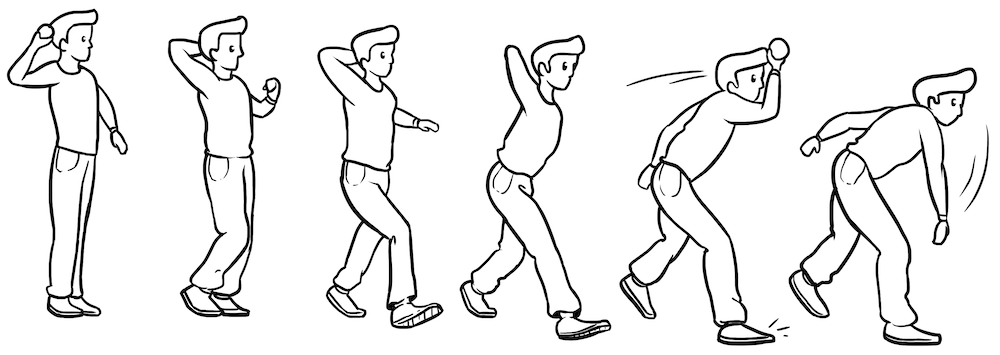
\includegraphics[width=0.9\linewidth]{static/images/man-ot/ot2.png} \\
\hline
\textbf{Level 3$\rightarrow$} The movement involves a trunk rotation to one side and a slight step forward with the opposite leg. & \textbf{Level 4$\rightarrow$} The trunk rotates to the side with a long contralateral step forward (at least half the performer's height). \\
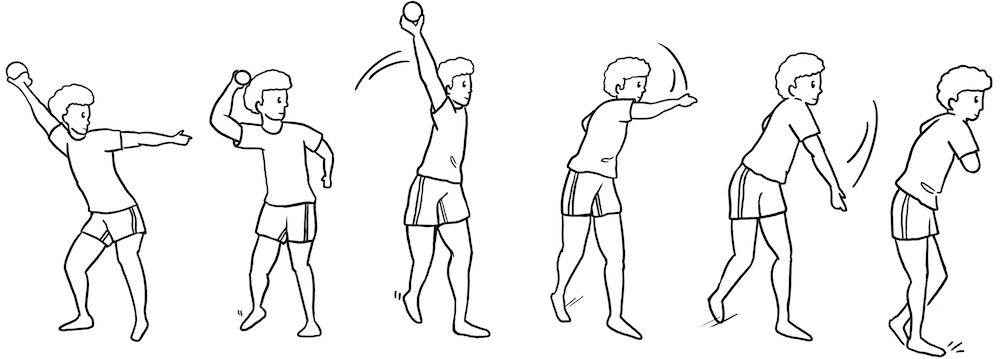
\includegraphics[width=0.9\linewidth]{static/images/man-ot/ot3.png} & 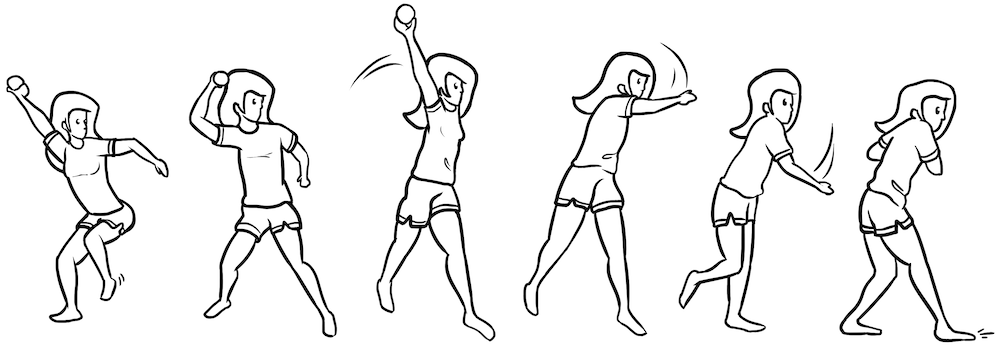
\includegraphics[width=0.9\linewidth]{static/images/man-ot/ot4.png} \\
\hline
\end{tabular}
\end{tabular}

\newpage

\setlength{\tabcolsep}{3pt}
\renewcommand{\arraystretch}{1.6}
\small
\vspace*{.5em} % Add vertical space after the header before the first table

% ---------------- Table 1 ----------------
\begin{tabular}{|p{5.5cm}|c|p{5.5cm}|c|c|*{9}{p{1.07cm}|}}
\hline
\multicolumn{5}{|c|}{\multirow{2}{*}{\centering \textbf{Manipulative: Kick}}} & \multicolumn{9}{c|}{\textbf{Student ID}} \\ 
\cline{6-14}
\multicolumn{5}{|c|}{} & & & & & & & & & \\
\hline
\multirow{4}{5.5cm}{\raggedright {\footnotesize Did the child take a long stride/leap before ball contact?}} 
& \multirow{2}{*}{\footnotesize Y} 
& \multirow{2}{5.5cm}{\raggedright {\footnotesize Did the placement foot move forward following ball contact?}} & {\footnotesize Y} & {\footnotesize Level 4} & & & & & & & & & \\
\cline{4-14}
& & & {\footnotesize N} & {\footnotesize Level 3} & & & & & & & & & \\
\cline{2-14}
& \multirow{2}{*}{\footnotesize N} & \multirow{2}{5.5cm}{\raggedright {\footnotesize Did the child fail to step toward the ball?}} & {\footnotesize Y} & {\footnotesize Level 2} & & & & & & & & & \\
\cline{4-14}
& & & {\footnotesize N} & {\footnotesize Level 1} & & & & & & & & & \\
\hline
\end{tabular}

\vspace{.5em}

% ---------------- Table 2 ----------------
\begin{tabular}{@{}l@{\hspace{1.5em}}l@{}}
% LEFT COLUMN: bullet lists with adjusted vertical placement
\small
\raisebox{0pt}[0pt][0pt]{%
\begin{tabular}[t]{@{}p{8.4cm}@{}}
\vspace*{1ex} % small vertical nudge
\textbf{Set up} \\[-1em]
\begin{itemize}
    \item Tape a line on the floor 15 feet from the wall.
    \item Place a medium-sized playground or soccer ball 3 feet ahead of the taped line.
    \item Stand about 10 feet from the performer to get a side view of the action.
\end{itemize}

\vspace{0.4em}
\textbf{Directions for performers} \\[-1em]
\begin{itemize}
    \item I want to see you kick the ball.
    \item Kick it as hard as you can to hit the wall.
    \item Start behind the line.
    \item After you kick, go get the ball and bring it back.
    \item Then do it three more times.
    \item Watch as I demonstrate.
\end{itemize}

\vspace{0.4em}
\textbf{Notes for examiners} \\[-1em]
\begin{itemize}
    \item Give the performer four trials (the first trial is for practice only).
    \item Replace the ball to the same position after each trial.
\end{itemize}
\end{tabular}
}
&
% RIGHT COLUMN: full boxed 2x2 layout
\begin{tabular}[t]{|p{7.9cm}|p{7.9cm}|}
\hline
\textbf{Level 1$\rightarrow$} Performer attempts to strike the ball with the feet but misses and does not make contact. & \textbf{Level 2$\rightarrow$} The kicking leg does not show a preparatory backswing and pushes the ball forward rather than showing a kicking action. \\
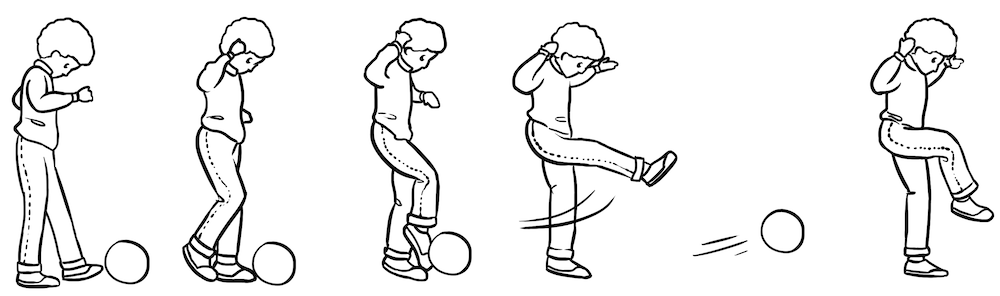
\includegraphics[width=0.9\linewidth]{static/images/man-kick/ki1.png} & 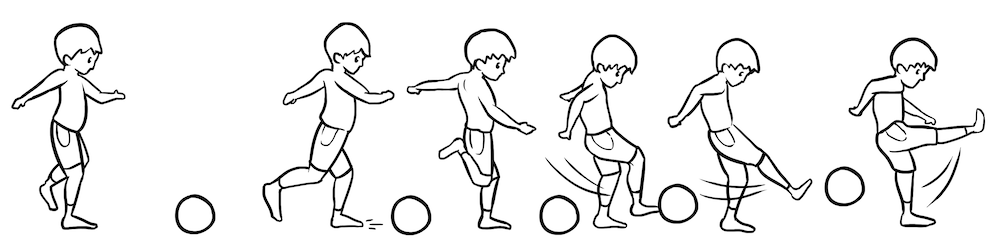
\includegraphics[width=0.9\linewidth]{static/images/man-kick/ki2.png} \\
\hline
\textbf{Level 3$\rightarrow$} The kicking leg backswings before contact, but the non-kicking foot is placed well ahead of the ball at impact. & \textbf{Level 4$\rightarrow$} The kicking leg backswings, and the non-kicking foot is placed even with or slightly behind the ball at impact. \\
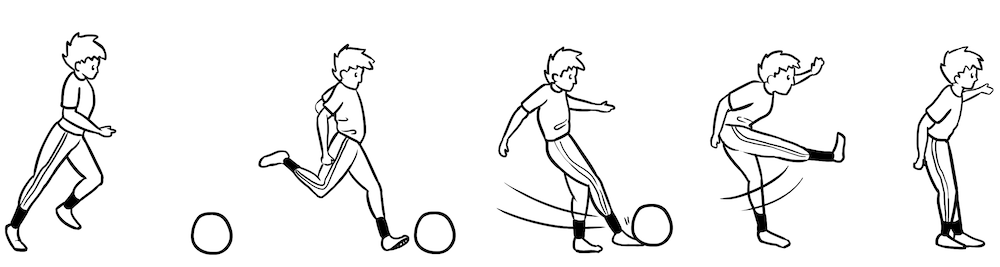
\includegraphics[width=0.9\linewidth]{static/images/man-kick/ki3.png} & 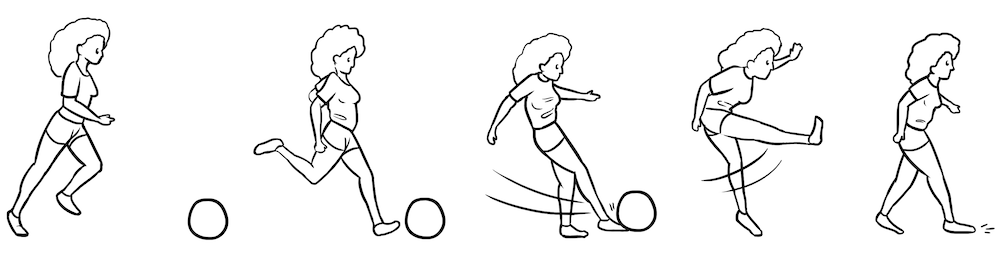
\includegraphics[width=0.9\linewidth]{static/images/man-kick/ki4.png} \\
\hline
\end{tabular}
\end{tabular}

\newpage

\setlength{\tabcolsep}{3pt}
\renewcommand{\arraystretch}{1.6}
\small
\vspace*{.5em} % Add vertical space after the header before the first table

% ---------------- Table 1 ----------------
\begin{tabular}{|p{5.5cm}|c|p{5.5cm}|c|c|*{9}{p{1.07cm}|}}
\hline
\multicolumn{5}{|c|}{\multirow{2}{*}{\centering \textbf{Manipulative: Hand Dribble}}} & \multicolumn{9}{c|}{\textbf{Student ID}} \\ 
\cline{6-14}
\multicolumn{5}{|c|}{} & & & & & & & & & \\
\hline
\multirow{4}{5.5cm}{\raggedright {\footnotesize Did the ball bounce in front/outside of the preferred foot?}} 
& \multirow{2}{*}{\footnotesize Y} 
& \multirow{2}{5.5cm}{\raggedright {\footnotesize Was the child able to keep control without using vision?}} & {\footnotesize Y} & {\footnotesize Level 4} & & & & & & & & & \\
\cline{4-14}
& & & {\footnotesize N} & {\footnotesize Level 3} & & & & & & & & & \\
\cline{2-14}
& \multirow{2}{*}{\footnotesize N} & \multirow{2}{5.5cm}{\raggedright {\footnotesize Did the child ever lose total control of the ball?}} & {\footnotesize Y} & {\footnotesize Level 1} & & & & & & & & & \\
\cline{4-14}
& & & {\footnotesize N} & {\footnotesize Level 2} & & & & & & & & & \\
\hline
\end{tabular}

\vspace{.5em}

% ---------------- Table 2 ----------------
\begin{tabular}{@{}l@{\hspace{1.5em}}l@{}}
% LEFT COLUMN: bullet lists with adjusted vertical placement
\small
\raisebox{0pt}[0pt][0pt]{%
\begin{tabular}[t]{@{}p{8.4cm}@{}}
\vspace*{1ex} % small vertical nudge
\textbf{Set up} \\[-1em]
\begin{itemize}
    \item Tape a 4'x4' square on the floor to designate personal space.
    \item Stand about 6 feet from the examinee.
    \item Place a bucket of soccer balls 3 feet before the kicking line.
\end{itemize}

\vspace{0.4em}
\textbf{Directions for performers} \\[-1em]
\begin{itemize}
    \item I want to see you dribbling a basketball with one hand.
    \item Try to stay inside the square while dribbling the ball.
    \item If the ball goes out of bounds, pick it up, return inside the square, and re-start.
    \item I will tell you when to stop.
    \item Watch as I demonstrate.
\end{itemize}

\vspace{0.4em}
\textbf{Notes for examiners} \\[-1em]
\begin{itemize}
    \item Inquire about the child's preferred foot
    \item Give the performer a practice trial (about 5 seconds).
    \item Time the child's dribbling for 15 seconds using a stopwatch. Stop if the ball goes out, and resume when dribbling restarts.
    \item Children controlling the ball without looking show vision-independent control; otherwise, they're at Level 3.
\end{itemize}
\end{tabular}
}
&
% RIGHT COLUMN: full boxed 2x2 layout
\begin{tabular}[t]{|p{7.9cm}|p{7.9cm}|}
\hline
\textbf{Level 1$\rightarrow$} The child struggles to control the ball as it bounces erratically and loses control at least once. & \textbf{Level 2$\rightarrow$} Despite a lack of control, the child bounces the ball continuously for 15 seconds. \\
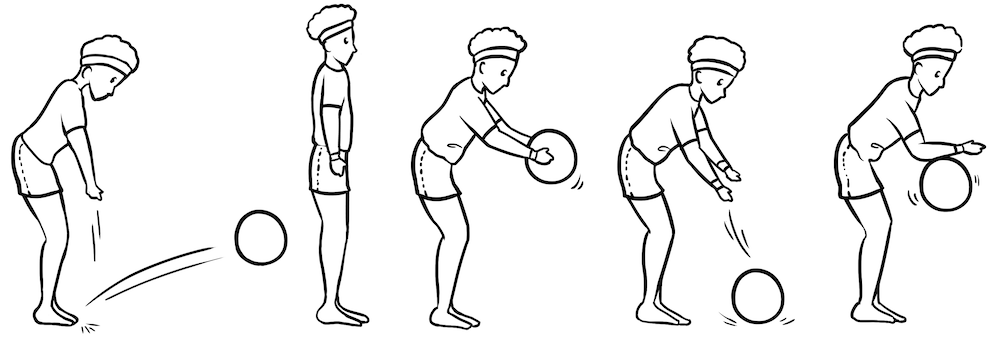
\includegraphics[width=0.9\linewidth]{static/images/man-dribble/dr1.png} & 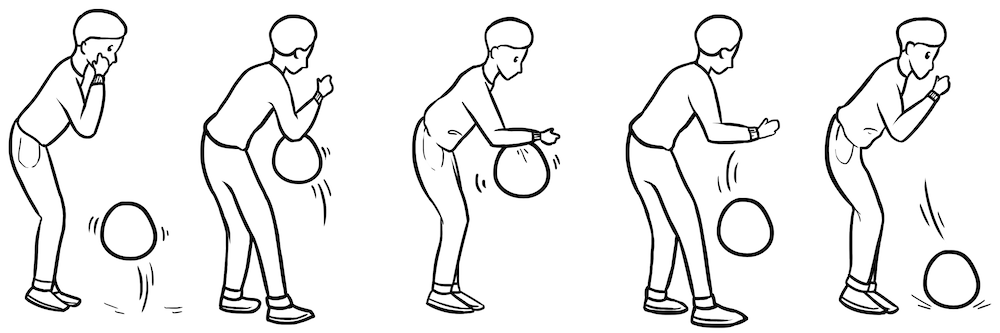
\includegraphics[width=0.9\linewidth]{static/images/man-dribble/dr2.png} \\
\hline
\textbf{Level 3$\rightarrow$} Vision is used to maintain ball control. Bounces occur in front of or to the outside of the child's preferred foot, and the child has more control over the ball. & \textbf{Level 4$\rightarrow$} Control is clear, and the child does not rely on vision to maintain ball control. \\
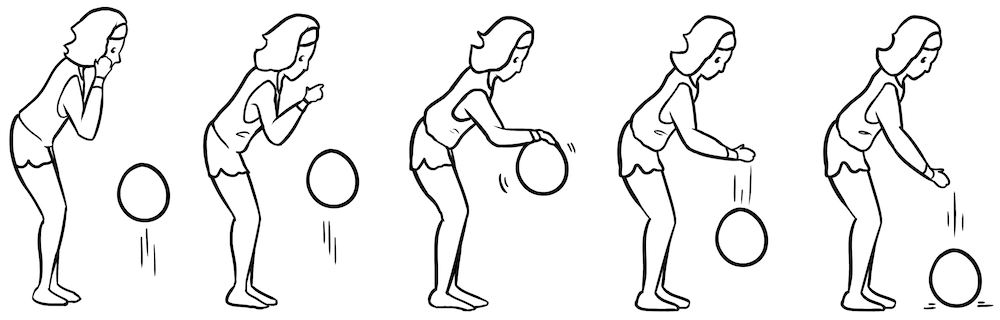
\includegraphics[width=0.9\linewidth]{static/images/man-dribble/dr3.png} & 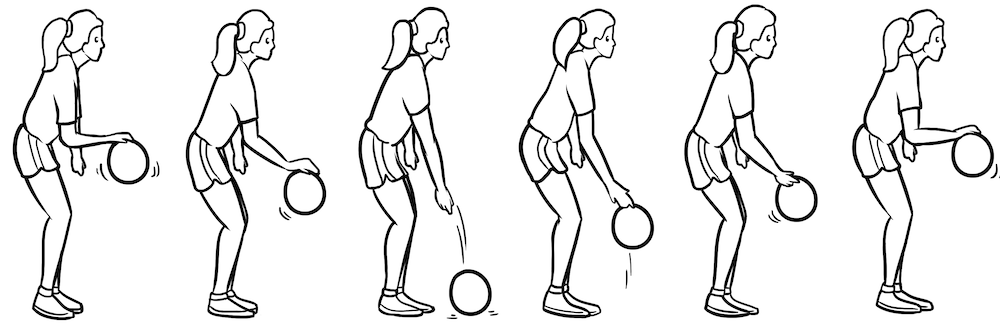
\includegraphics[width=0.9\linewidth]{static/images/man-dribble/dr4.png} \\
\hline
\end{tabular}
\end{tabular}

\newpage

\setlength{\tabcolsep}{3pt}
\renewcommand{\arraystretch}{1.6}
\small
\vspace*{.5em} % Add vertical space after the header before the first table

% ---------------- Table 1 ----------------
\begin{tabular}{|p{5.5cm}|c|p{5.5cm}|c|c|*{9}{p{1.07cm}|}}
\hline
\multicolumn{5}{|c|}{\multirow{2}{*}{\centering \textbf{Manipulative: Catch}}} & \multicolumn{9}{c|}{\textbf{Student ID}} \\ 
\cline{6-14}
\multicolumn{5}{|c|}{} & & & & & & & & & \\
\hline
\multirow{4}{5.5cm}{\raggedright {\footnotesize Was the ball caught using only hands without touching any other body part?}} 
& \multirow{2}{*}{\footnotesize Y} 
& \multirow{2}{5.5cm}{\raggedright {\footnotesize Did the hands move well-timed and synchronized while catching the ball?}} & {\footnotesize Y} & {\footnotesize Level 4} & & & & & & & & & \\
\cline{4-14}
& & & {\footnotesize N} & {\footnotesize Level 3} & & & & & & & & & \\
\cline{2-14}
& \multirow{2}{*}{\footnotesize N} & \multirow{2}{5.5cm}{\raggedright {\footnotesize Did the child trap the ball against the chest?}} & {\footnotesize N} & {\footnotesize Level 2} & & & & & & & & & \\
\cline{4-14}
& & & {\footnotesize Y} & {\footnotesize Level 1} & & & & & & & & & \\
\hline
\end{tabular}

\vspace{.5em}

% ---------------- Table 2 ----------------
\begin{tabular}{@{}l@{\hspace{1.5em}}l@{}}
% LEFT COLUMN: bullet lists with adjusted vertical placement
\small
\raisebox{0pt}[0pt][0pt]{%
\begin{tabular}[t]{@{}p{8.4cm}@{}}
\vspace*{1ex} % small vertical nudge
\textbf{Set up} \\[-1em]
\begin{itemize}
    \item Tape a 4'x4' on the floor to designate personal space.
    \item Stand about 6 feet from the child.
\end{itemize}

\vspace{0.4em}
\textbf{Directions for performers} \\[-1em]
\begin{itemize}
    \item I want to see you catch a ball with two hands.
    \item Stand anywhere inside the square.
    \item Watch as I demonstrate.
\end{itemize}

\vspace{0.4em}
\textbf{Notes for examiners} \\[-1em]
\begin{itemize}
    \item Give the performer four trials (the first trial is for practice only).
    \item Use an underhand toss and toss the ball at the child's chest level.
    \item Repeat any attempt that results from a bad toss (too high/low or to the sides).
    \item Only assess consistency on the three "valid" tosses.
    \item If the ball is caught with hands and later brought against the chest, this indicates Level 2.
    \item A behavior is considered present (answering YES) if observed in at least two trials.
\end{itemize}
\end{tabular}
}
&
% RIGHT COLUMN: full boxed 2x2 layout
\begin{tabular}[t]{|p{7.9cm}|p{7.9cm}|}
\hline
\textbf{Level 1$\rightarrow$} The child uses a scooping action to secure the ball against the chest. & \textbf{Level 2$\rightarrow$} Following a successful catch, the ball is not secured against the chest but touches a body part other than the hands. \\
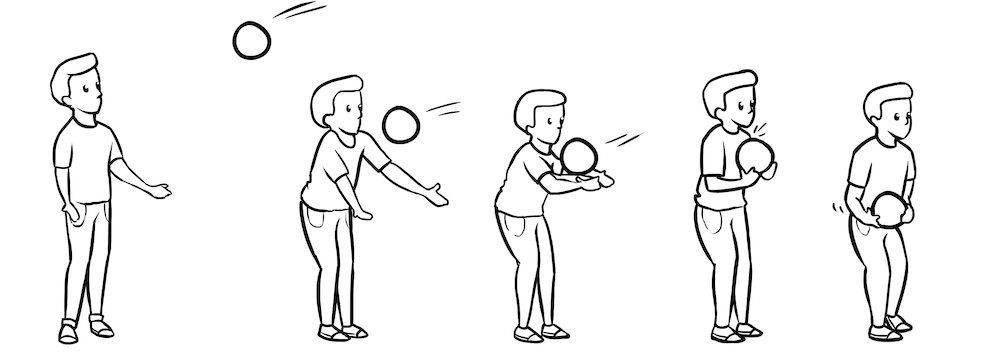
\includegraphics[width=0.9\linewidth]{static/images/man-catch/ca1.png} & 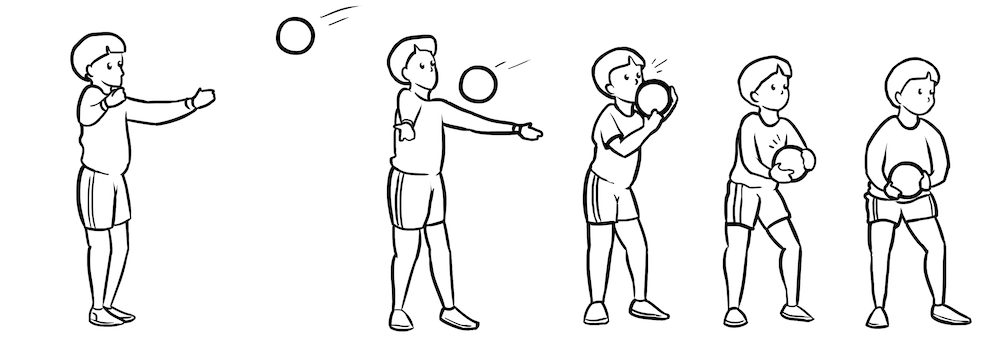
\includegraphics[width=0.9\linewidth]{static/images/man-catch/ca2.png} \\
\hline
\textbf{Level 3$\rightarrow$} The action lacks coordination, with the ball making contact only with the hands. Players often extend their arms and/or turn their faces to the side. & \textbf{Level 4$\rightarrow$} Action is well-timed with the simultaneous motion of hands. \\
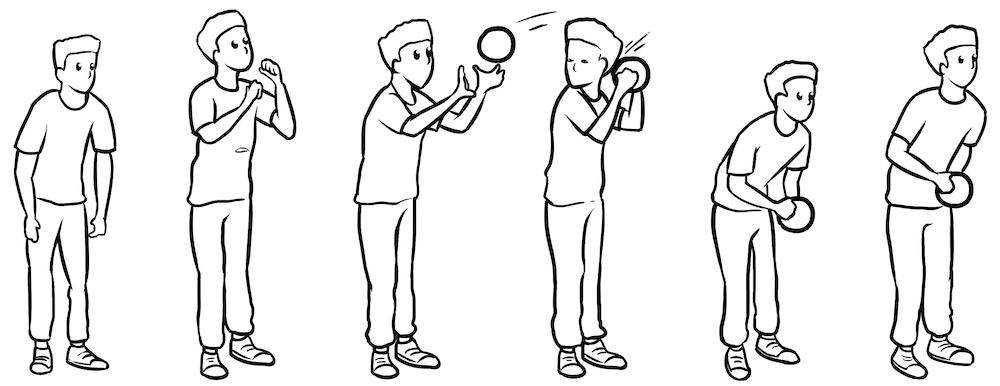
\includegraphics[width=0.9\linewidth]{static/images/man-catch/ca3.png} & 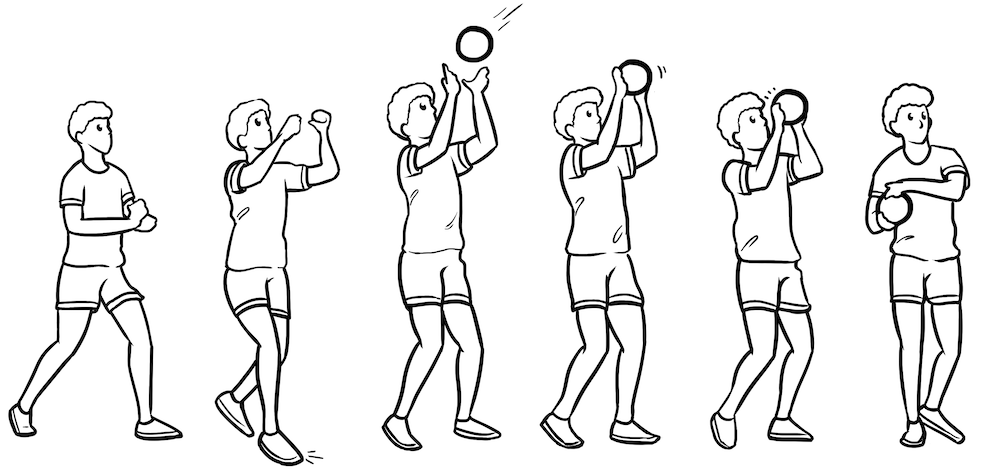
\includegraphics[width=0.9\linewidth]{static/images/man-catch/ca4.png} \\
\hline
\end{tabular}
\end{tabular}

\newpage

\setlength{\tabcolsep}{3pt}
\renewcommand{\arraystretch}{1.6}
\small
\vspace*{.5em} % Add vertical space after the header before the first table

% ---------------- Table 1 ----------------
\begin{tabular}{|p{5.5cm}|c|p{5.5cm}|c|c|*{9}{p{1.07cm}|}}
\hline
\multicolumn{5}{|c|}{\multirow{2}{*}{\centering \textbf{Manipulative: Strike}}} & \multicolumn{9}{c|}{\textbf{Student ID}} \\ 
\cline{6-14}
\multicolumn{5}{|c|}{} & & & & & & & & & \\
\hline
\multirow{4}{5.5cm}{\raggedright {\footnotesize Did the swing follow a full arc in a horizontal plane?}} 
& \multirow{2}{*}{\footnotesize Y} 
& \multirow{2}{5.5cm}{\raggedright {\footnotesize Did the body weight shift from one leg to the other during movement?}} & {\footnotesize Y} & {\footnotesize Level 4} & & & & & & & & & \\
\cline{4-14}
& & & {\footnotesize N} & {\footnotesize Level 3} & & & & & & & & & \\
\cline{2-14}
& \multirow{2}{*}{\footnotesize N} & \multirow{2}{5.5cm}{\raggedright {\footnotesize Was the bat's motion on a downward plane from back to front?}} & {\footnotesize N} & {\footnotesize Level 2} & & & & & & & & & \\
\cline{4-14}
& & & {\footnotesize Y} & {\footnotesize Level 1} & & & & & & & & & \\
\hline
\end{tabular}

\vspace{.5em}

% ---------------- Table 2 ----------------
\begin{tabular}{@{}l@{\hspace{1.5em}}l@{}}
% LEFT COLUMN: bullet lists with adjusted vertical placement
\small
\raisebox{0pt}[0pt][0pt]{%
\begin{tabular}[t]{@{}p{8.4cm}@{}}
\vspace*{1ex} % small vertical nudge
\textbf{Set up} \\[-1em]
\begin{itemize}
    \item Tape a 4'x4' square on the floor 20 feet from the wall.
    \item Stand slightly to the side (about 12 feet), facing the performer.
    \item Invert the position (the child faces the opposite wall/open space) if left-handed.
\end{itemize}

\vspace{0.4em}
\textbf{Directions for performers} \\[-1em]
\begin{itemize}
    \item I want to see you strike a ball tossed in your direction.
    \item Try to stay inside the square, but you are free to move as the ball approaches.
    \item Strike the ball against the wall/open space.
    \item Watch as I demonstrate.
\end{itemize}

\vspace{0.4em}
\textbf{Notes for examiners} \\[-1em]
\begin{itemize}
    \item Give the performer 4 trials (1st trial is for practice only).
    \item Use an underhand toss.
    \item Toss the ball at the child's hip level.
    \item Repeat any attempt that results from a bad toss (too high/low or to the sides).
    \item Only assess consistency on the three "valid" tosses.
    \item A behavior is considered present (answering YES) if observed in at least two trials.
\end{itemize}
\end{tabular}
}
&
% RIGHT COLUMN: full boxed 2x2 layout
\begin{tabular}[t]{|p{7.9cm}|p{7.9cm}|}
\hline
\textbf{Level 1$\rightarrow$} The arm action is from back to front and resembles a vertical chopping motion. & \textbf{Level 2$\rightarrow$} The motion occurs on the horizontal plane, but the action is limited in its amplitude. Often, the bat is held in front of the body. \\
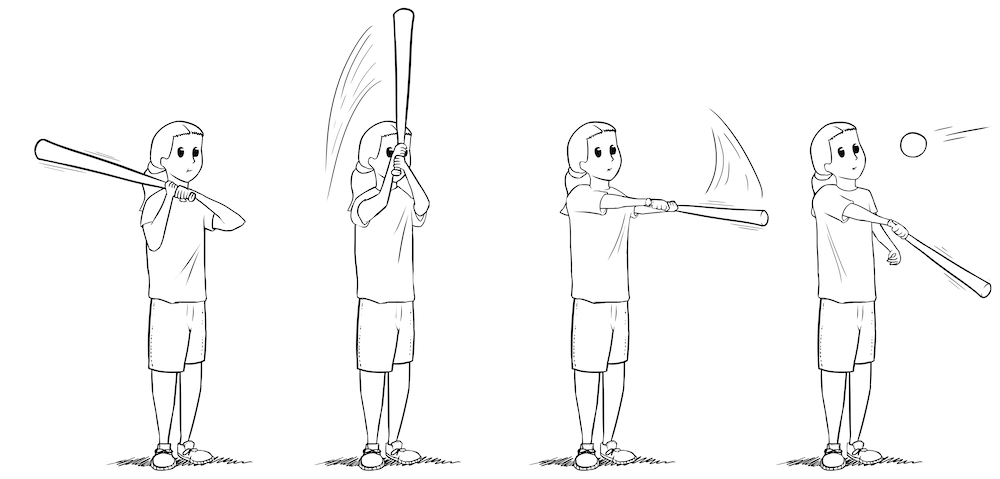
\includegraphics[width=0.9\linewidth]{static/images/man-strike/st1.png} & 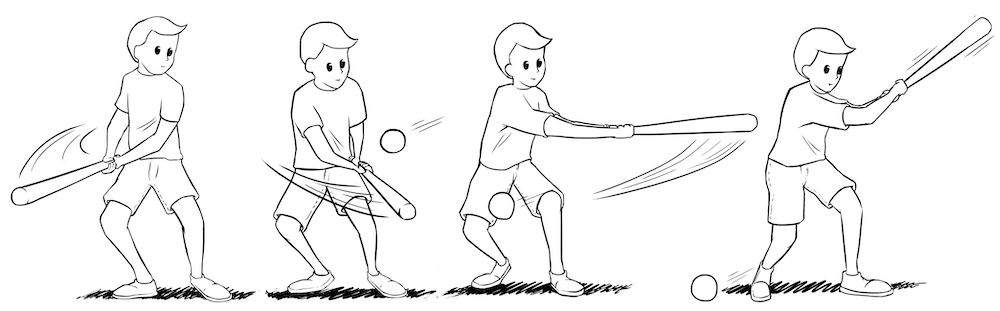
\includegraphics[width=0.9\linewidth]{static/images/man-strike/st2.png} \\
\hline
\textbf{Level 3$\rightarrow$} The strike does occur in a long (full arc) horizontal plan, but there is no body weight transfer. & \textbf{Level 4$\rightarrow$} Same as Level 3, but now there is a transfer of body weight in the direction of the strike, which occurs from one leg to the other leg. \\
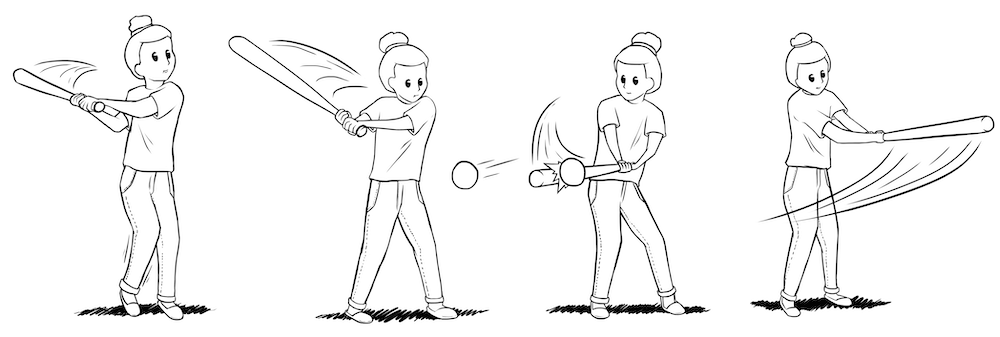
\includegraphics[width=0.9\linewidth]{static/images/man-strike/st3.png} & 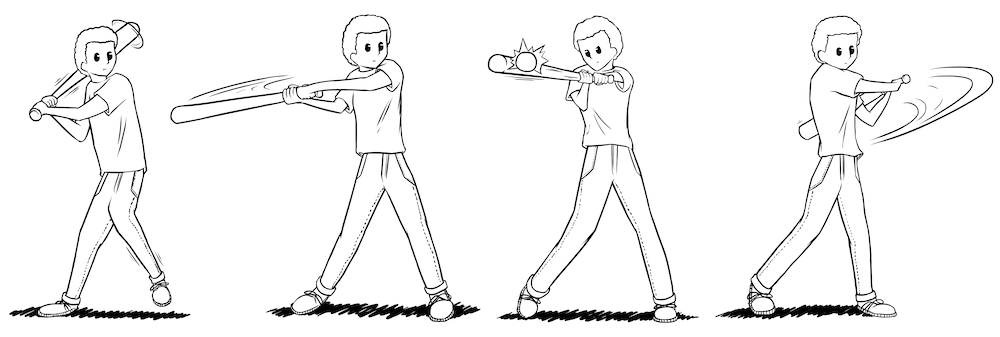
\includegraphics[width=0.9\linewidth]{static/images/man-strike/st4.png} \\
\hline
\end{tabular}
\end{tabular}




\end{document}
